\documentclass{article}
\usepackage{graphicx} % Required for inserting images
\usepackage{amsmath}
\usepackage{booktabs} % For better table lines
\usepackage{array} % For better column control
\usepackage{amssymb}
\usepackage{float} % for moving graphics around 
\usepackage{caption} 

\begin{document}

% Title Page
\begin{titlepage}
    \centering
    \vspace*{1in} % Vertical space at the top of the page
    {\LARGE \textbf{Econometrics (ECON211A)}} \\[0.5cm]
    {\LARGE Allegra Saggese} \\ [.5cm] % author
    {\large 2024-25 UCSC Economics PhD} \\ [1.5 cm] 
    {\large Fall 2024} \\[.25cm] % quarter
    {\large Julian Martinez-Iriarte} \\[.25cm]
    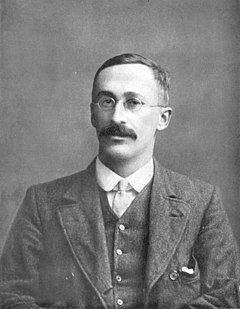
\includegraphics[width=0.4\textwidth]{William_Sealy_Gosset.jpg} 
    \vfill
    \end{titlepage}

% TOC
\clearpage
\pagestyle{empty} % ensures no headers on this page
\noindent \textbf{Last updated: \today} 
\vspace{0.5cm} % Adjust space before the TOC
\tableofcontents
\clearpage % next page
\pagestyle{plain} %remove headers



\section{Probability Theory and Random Variables}
% under each section - should put roughly the corresponding chapter in Casella-Berger as it was quite close to the book 
1. If \(A\) and \(B\) are pairwise disjoint, then the union of all partitions is the sum of all probabilities of each partition.
\begin{enumerate}
    \item Instead of checking for the satisfaction of all three probability axioms of all probability functions, we can use the following theorem: If \(S\) is a finite set, \(B\) is a sigma algebra of the subsets of \(S\), and \(p_1, \ldots, p_n\) are nonnegative numbers that sum to 1. Then for any \(A \in B\), \(P(A) = \sum p_i\) for all \(i : s_i \in A\).
    \item From the axioms of probability, we can infer other important pieces of information, such as: \(P(\text{null}) = 0\), \(P(A) \leq 1\), \(P(A^C) = 1 - P(A)\), and \(P(A \cup A^C) = P(S) = 1\) (or \(P(A \cup A^C) = P(A) + P(A^C)\)).
    \item Theorems for probability functions—more formalized than the above identities—include:
   \begin{enumerate}
       \item \(P(B \cap A^C) = P(B) - P(A \cap B)\)
       \item \(P(A \cup B) = P(A) + P(B) - P(A \cap B)\)
       \item If \(A \subseteq B\), then \(P(A) \leq P(B)\)
       \item Bonferroni's Inequality: Since \(P(A \cup B) \leq 1\), then \(P(A \cap B) \geq P(A) + P(B) - 1\). This is useful to characterize the probability intersection of \(A\) and \(B\) in terms of the individual probabilities. This allows us to bound the probability of simultaneous events in terms of just \(P(A)\) and \(P(B)\).
       \item \(P(A) = \sum P \cap C_i\) for any partition \(C_1, C_2, \ldots\) where the union of the partitions will be the subset \(S\). This is true because \(A\) with the intersection of the unions of \(C_i\) are equal to \(A \cap S\). Then, we know all \(C_i\) are pairwise disjoint, making it possible to use the distributive law to show that for each intersection of \(A\) with some \(C_i\), we get the probability of the total of \(A\).
       \item Boole's Inequality: \(P\left(\bigcup A_i\right) \leq \sum P(A_i)\) where \(A_i\) are disjoint, thus \(A_i \subseteq C A_i\).
   \end{enumerate}
\end{enumerate}

\textbf{For midterm: we can skip counting in the textbook!} \\ 
\vspace{3mm}
3. Conditional probability: 
\[
P(A|B) = \frac{P(A \cap B)}{P(B)}
\]
This is because \(B\) becomes the sample space (so \(P(B|B) = 1\)).

4. Other formulas for conditional probability:
   \begin{enumerate}
       \item \(P(A \cap B) = P(B|A) \cdot P(A)\), note: this holds symmetry, so we can rearrange the conditional probability. It is equivalent to \(P(B \cap A) = P(A|B) \cdot P(B)\)
       \item Rearranging, we introduce \textbf{Baye's Rule}: \(P(A | B) = \frac{P(B|A) \cdot P(A)}{P(B)}\)
   \end{enumerate}

5. Bayes' Rule:
\[
P(A_i|B) = \frac{P(B|A_i) \cdot P(A_i)}{\sum P(B|A_j) \cdot P(A_j)}
\]

6. Statistical independence: 
\[
P(A \cap B) = P(A) \cdot P(B)
\]
when two events are statistically independent. This means the conditional probability is equal to zero.
   \begin{enumerate}
       \item If \(A\) and \(B\) are independent, the following pairs are also independent: 
           \begin{enumerate}
               \item \(A\) and \(B^c\)
               \item \(A^c\) and \(B\)
               \item \(A^c\) and \(B^c\)
           \end{enumerate}
   \end{enumerate}

7. Random variables: Random variables are functions from a sample space \(S\) into real numbers. It's important to frame random variables correctly, particularly that 
\[
P_X(X = x_i) = P(\{s_j \in S: X(s_j) = x_i\})
\]
   \begin{enumerate}
       \item The range of the random variable is all potential values that the random variable can take on. For example, in a random variable defined as the number of heads in a coin toss that occurs three times, the range is \{0, 1, 2, 3\} because you can have from zero to three heads appear in the coin toss. Then you can set \(P(X=x)\), where \(x_i, \ldots, x_n = i = 0, \ldots, 3\).
       \item Continuous random variables: If \(F_X(x)\) is a continuous function of \(x\) (similarly, if \(f_X(x)\) is a step function of \(x\), then the random variable is discrete).
       \item Random variables' probability distribution is determined completely by \(F_X\). It's important to see the relationship between random variables and their cumulative distribution function.
       \item Identical distribution of random variables: 
           \begin{enumerate}
               \item \(X, Y\) are identically distributed if for every set \(A\), \(P(X \in A) = P(Y \in A)\), this does not imply that they are the same random variable, but that they have an identical distribution. This can also be written as \(F_X(x) = F_Y(x)\) for every \(x\).
           \end{enumerate}
   \end{enumerate}

8. Distribution, density, and mass functions:
   \begin{itemize}
       \item Cumulative distribution function (CDF): \(F_X(x)\), defined as \(P_X(X \leq x)\) for all \(x\). CDF measures the cumulative probability up until the random variable \(X\). The following conditions must be met:
           \begin{enumerate}
               \item \(\lim_{x \to -\infty} F(x) = 0\) and \(\lim_{x \to \infty} F(x) = 1\)
               \item \(F(x)\) is a nondecreasing function of \(x\) 
               \item \(F(x)\) is right continuous. That is, for every number \(x_0\), the limit as \(x\) approaches \(x_0\) of \(F(x) = F(x_0)\)
           \end{enumerate}
       \item Probability mass function (discrete) or probability density function \(f_X(x)\) is the probability of a random variable at any point \(x\).
           \begin{enumerate}
               \item Discrete: \(f_X(x) = P(X = x)\) for all \(x\)
               \item Continuous: \(P(X \leq x) = F_X(x) = \int_{-\infty}^{x} f_X(t) dt\), using the fundamental theorem of calculus, we have \(\frac{d}{dx}F_X(x) = f_X(x)\) (so the derivative of the CDF at some \(x\) is the PDF).
               \item To be a PDF, \(f_X(x)\) must satisfy the following: 
                   \begin{enumerate}
                       \item \(F_X(x) \geq 0\) for all \(x\)
                       \item The sum of \(F_X(x) = 1\) (discrete) or the integral of \(f_X(x) \, dx = 1\) (continuous case), this is the cumulative distribution function property
                       \item Remember that $P(X=c) = 0$ for all density functions, as there is no particular probability at a certain point
                   \end{enumerate}
           \end{enumerate}
   \end{itemize}

9. Counting: The number of partial derivatives is an exponential function, dependent on the number of variables. For example, a function has \(n^k\) partial derivatives, where \(n\) is the number of variables, and \(k\) is the count of partial derivatives you are taking (if you have a three-variable function to the fourth partial derivative, then \(n = 3\), \(k = 4\), and \(3^4 = 81\)). This arises from the property that variables are independent.

\section{Transformations and Expectations}

\begin{enumerate}
    \item Law of iterated expectations (LIE) where \( E[U] = E[E[U|X]] \). Essentially, if you take the expected value of the conditional expectations, you are summing the conditional expectations. Therefore, you end up back in the unconditional case. 
    \item Inverse mapping of a random variable
    \begin{enumerate}
        \item If we have another variable, \( Y \), we can write it as \( g(x) = Y \), with probabilistic behavior in terms of \( x \). So \( P(Y \in A) = P(g(X) \in A) \).
        \item \( Y \) has a new sample space, so \( g(x): X \to Y \), which is an inverse mapping, so \( g^{-1}(A): \{ x \in X: g(x) \in A \} \).
        \item \( P(Y \in A) = P(X \in g^{-1}(A)) = \) the probability distribution of \( Y \).
        \item For the transformation, it is best to use the sample space forms:
        \begin{enumerate}
            \item \( X = \{ x: f_X(x) > 0 \} \)
            \item \( Y = \{ y: y = g(x) \text{ for some } x \in X \} \)
        \end{enumerate}
    \end{enumerate}
    
    \item Support (set): The support is a set where the PDF of a random variable, \( X \), is positive and zero elsewhere. Supports are attached to distributions (PMF or PDF).
    \begin{enumerate}
        \item Useful to know if \( g(x) \) is monotone (increasing or decreasing), because then the \( y \) that is paired with \( x \) can only be paired with one value of \( x \). Such is a function that is strictly one-to-one.
        \item Theorem (for supports): Let \( X \) have CDF \( F_X(x) \) and \( Y = g(X) \). Let \( X, Y \) be defined as the typical sample spaces. Then:
        \begin{enumerate}
            \item If \( g \) is increasing on \( X \), \( F_Y(y) = F_X(g^{-1}(y)) \) for \( y \in Y \).
            \item If \( g \) is a decreasing function on \( X \) and \( X \) is a continuous random variable, then \( F_Y(y) = 1 - F_X(g^{-1}(y)) \) for \( y \in Y \).
        \end{enumerate}
        \item Steps to getting the support:
        \begin{enumerate}
            \item Firstly, look at the sample space, \( X \). Know \( x \in X \). And there exists some function, \( y = g(X) \) (it’s a transformation on the random variable), which we will use to get the support.
            \item Second, the support is then the set where the PDF of \( X \) is positive on the sample set, \( X \).
            \item Third, we check to see if \( g(x) \) is strictly increasing/decreasing to determine the function for how to write the CDF of the support.
            \item Then, integrate from \( g^{-1}(y) \) to infinity for \( f_X(x) \, dx \), as this captures all values of \( x \in X \) where \( x \leq g^{-1}(y) \).
            \item Plug in the bounds of the \( x \) set into \( g(x) \) to get the range for \( Y \), or the support for \( Y \).
            \item Rearrange \( y = g(X) = \) some function to get it in terms of \( x \).
            \item Then plug that \( x \) value into \( g^{-1}(y) \) for \( y \). So you get \( F_Y(y) \).
        \end{enumerate}
        \item Theorem for getting PDF of \( Y \) (where \( X \) has a PDF, \( Y = g(X) \), \( g \) is monotone, \( X,Y \) are sample spaces, and the PDF of \( X \) is continuous, the sample space \( X \) is continuous and the inverse of \( g \) is continually differentiable on \( Y \)). Then the PDF is:
        \begin{enumerate}
            \item \( f_Y(y) = \frac{d}{dy} F_Y(y) = f_X(g^{-1}(y)) \frac{d}{dy} g^{-1}(y) \) if increasing.
            \item \( f_Y(y) = \frac{d}{dy} F_Y(y) = -f_X(g^{-1}(y)) \frac{d}{dy} g^{-1}(y) \) if decreasing.
        \end{enumerate}
        \item One important case is if \( g(X) = x^2 \), monotone on \((- \infty, 0)\) and on \((0, \infty)\), and \( Y = (0, \infty) \), the PDF of \( Y \) is the chi-squared distribution with degree of one freedom.
    \end{enumerate}

    \item Theorem: If \( F \) has a continuous CDF \( F_X(x) \) and a random variable \( Y = F_X(X) \), then \( Y \) is uniformly distributed on \((0,1)\) for  \( P(Y \leq y) = y \), for \( 0 < y < 1 \).

    \item Expected value and conditional expected values for random variables
    \begin{enumerate}
        \item Cauchy random variables do not have expected values, as \( E[X] = \infty \).
        \item Properties of expected values (4) that are important.
        \item Minimizer function for the random variable and some constant, where you want to minimize \( b E(X-b)^2 = E(X - E(X))^2 \).
        \item To calculate the $E[X]$ from a density function $F_x(X)$ you need the following formula: $ \int_{-\infty}^{\infty} x f_x(x) \, dx $

    \end{enumerate}

    \item Moment generating functions:
    \begin{enumerate}
        \item First moment (\(n = 1\)) is the expected value, and is \( E(X - \mu)^n \) where \( \mu = \mu^1 \) so the mean is the first moment. This is also known as the expected value of \( X \), \( E[X] \).
        \item \textbf{Variance:} Second moment (\(n = 2\)) is the variance, which gives a measure of the degree of spread of a distribution around its mean. The functional form is \( \text{Var}(X) = E(X - E[X])^2 \).
        \begin{enumerate}
            \item If \( X \) is a random variable with a finite variance, then for any constants \( a,b \): \( \text{Var}(aX + b) = a^2 \text{Var}(X) \).
            \item \(\text{Variance}\) can also be written as: \( \text{Var}(X) = E[X^2] - (E[X])^2 \).
        \end{enumerate}
        \item Moment generating function (MGF): 
        \[
        M_X(t) = E[e^{tX}],
        \]
        where if it is continuous it is the integral of \( e^{tx} f_X(x) \, dx \).
        \begin{enumerate}
            \item The \(n\)th moment is equal to the \(n\)th derivative of \(M_X(t)\) evaluated at \(t=0\).
        \end{enumerate}
        \item If \( F_X(x) \) and \( F_Y(y) \) are two CDFs whose moments exist, then:
        \begin{enumerate}
            \item If \( F_X \) and \( F_Y \) have bounded support, then \( F_X(u) = F_Y(u) \) for all \( u \) IFF \( E[X^r] = E[Y^r] \) for all integers \( r = 0, 1, 2, \ldots \).
            \item If the MGFs exist and \( M_X(t) = M_Y(t) \) for all \( t \) in some neighborhood of zero, then \( F_X(u) = F_Y(u) \) for all \( u \).
        \end{enumerate}
        \item For any constants \( a,b \), the MGF of the random variable \( aX + b \) is:
        \[
        M_{(aX + b)}(t) = e^{bt} M_X(at).
        \]
    \end{enumerate}

    \item Leibniz's rule: Chain rule for differentiating functions where the bounds of the integral are implicit functions. It requires taking the partial derivative of the bound multiplied by the function of the bound, then eventually differentiating the inside integral.

    \item Law of total variance: 
    \[
    \text{Var}(Y) = \text{Var}(E[Y|X]) + E[\text{Var}(Y|X)].
    \]
    \item Some important properties to remember when solving problems involving expectation, covariance, and independence:
\begin{itemize}
    \item  $E[XY|X] = E[X|X]E[Y|X] = XE[Y|X]$
     \item if $Cov(X, \epsilon) = 0, X$ and $\epsilon$ do not have to be independent. It is possible they are dependent. \textit{Only in the case where X, $\epsilon$ are jointly normally distributed, do we have that zero covariance implies independence.} For all $X \perp \epsilon$ then $Cov(X, \epsilon) = 0$
     \item For all $X \perp Y$ then $E[Y|X] = E[Y]$. There is no case where the conditional expectation is equal to the unconditional expectation where the theorem doesn't flow in the opposite direction. To prove use the definition of the the conditional density where 
     \vspace{-1mm}
     \begin{center}
              $f_xy(XY)/f_x(X) = f_x|y(X|Y)$
     \end{center}
\end{itemize}
\end{enumerate}

\section{Distributions}

\begin{table}[H]
    \centering
    \resizebox{0.95\textwidth}{!}{ % Resize to 80% of the text width
        \begin{tabular}{@{}>{\centering\arraybackslash}m{2cm} >{\centering\arraybackslash}m{2cm} >{\centering\arraybackslash}m{2cm} >{\centering\arraybackslash}m{2cm} >{\centering\arraybackslash}m{3cm} >{\centering\arraybackslash}m{3cm}@{}}
            \toprule
            \textbf{Distribution} & \textbf{Type} & \textbf{Mean} & \textbf{Variance} & \textbf{PDF} & \textbf{CDF} \\ \midrule
            Standard Normal & Continuous & $\mu=0$ & $\sigma^2=1$ & $f(x)=\frac{1}{\sqrt{2\pi}} e^{-\frac{x^2}{2}}$ & $F(x)=\frac{1}{2}\left(1+\text{erf}\left(\frac{x}{\sqrt{2}}\right)\right)$ \\ \hline
            Log-Normal & Continuous & $\mu$ (location parameter) & $\sigma^2$ (scale parameter) & $f(x)=\frac{1}{x\sigma\sqrt{2\pi}} e^{-\frac{(\ln x - \mu)^2}{2\sigma^2}}$ for $x>0$ & $F(x)=\Phi\left(\frac{\ln x - \mu}{\sigma}\right)$ \\ \hline
            Gamma & Continuous & $k\theta$ & $k\theta^2$ & $f(x)=\frac{x^{k-1} e^{-\frac{x}{\theta}}}{\theta^k\Gamma(k)}$ for $x>0$ & $F(x)=\frac{\gamma(k,\frac{x}{\theta})}{\Gamma(k)}$ \\ \hline
            Chi-Squared & Continuous & $k$ & $2k$ & $f(x)=\frac{1}{2^{k/2}\Gamma(k)} x^{(k/2)-1} e^{-x/2}$ for $x>0$ & $F(x)=\frac{\gamma(k/2,\frac{x}{2})}{\Gamma(k/2)}$ \\ \hline
            Uniform & Continuous & $\frac{a+b}{2}$ & $\frac{(b-a)^2}{12}$ & $f(x)=\frac{1}{b-a}$ for $a<x<b$ & $F(x)=\frac{x-a}{b-a}$ for $a<x<b$ \\ \hline
            Poisson & Discrete & $\lambda$ & $\lambda$ & $P(X=k)=\frac{\lambda^k e^{-\lambda}}{k!}$ for $k=0,1,2,\ldots$ & $F(k)=e^{-\lambda}\sum_{i=0}^{k} \frac{\lambda^i}{i!}$ \\ 
            \bottomrule
        \end{tabular}
    } % End of resizebox
    \caption{Summary of Different Probability Distributions}
    \label{tab:distributions}
\end{table}

%%%%%%%% STILL NEED TO FILL IN WITH DEFINITIONS - INCOMPLETE SECTION

\section{Conditional Distribution and Independence}

\begin{enumerate}
    \item \textbf{Conditional Probability}
    \begin{enumerate}
        \item Joint probability distribution \textit{times} marginal probability distribution.
        \item In the case that two random variables are independent, the conditional probability is simply the probability of the variable of interest.
    \end{enumerate}

    \item \textbf{Independence of \(X\), \(Y\) and Related Theorems for These Random Variables}

    \item \textbf{Marginal Probability Distribution Functions}
    \begin{enumerate}
        \item Formula.
    \end{enumerate}

    \item \textbf{Joint Probability Distribution Functions}
    \begin{enumerate}
        \item Including the fundamental theorem of calculus.
    \end{enumerate}

    \item \textbf{Mutually Independent Random Variables} 
    \begin{itemize}
        \item A stronger assumption than pairwise independence.
    \end{itemize}

    \item \textbf{Correlation and Covariation}

    \item \textbf{Proving the Normal Distribution}
    \begin{enumerate}
        \item Proof requires using the moment generating function \(M_z(t) = e^{t^2/2}\).
        \item Understand that when a normal distribution is transformed, it remains in the same 'normal distribution family,' i.e., \(N[0,1]\).
        \item If \(X \sim N(\mu, \sigma^2)\), then \(Z = \frac{X - \mu}{\sigma} \sim N(0,1)\).
        \item Recognize that \(Z\) retains the normal distribution (refer to Equation 4.47).
    \end{enumerate}

    \item \textbf{Chebyshev's Inequality}
    \begin{enumerate}
        \item The probability of some function \(g(x)\) being greater than or equal to \(r\) is bounded by \( \frac{\mathbb{E}[g(x)]}{r} \), i.e., 
        \[
        P(g(x) \geq r) \leq \frac{\mathbb{E}[g(x)]}{r}.
        \]
        \item This inequality refers to the tail behavior of the random variable, stating that the random variable, when sufficiently large, is bounded by the expected value.
        \item Example and proof should be well understood.
    \end{enumerate}

    \item {Definition of Variance, Covariance, and Correlation}
Definitions and properties should be clearly outlined.
\end{enumerate}


\begin{table}[H]
    \centering
    \caption{Function Types, Derivatives, and Integrals}
    \resizebox{0.95\textwidth}{!}{%
        \begin{tabular}{@{}>{\centering\arraybackslash}m{3cm} >{\centering\arraybackslash}m{3cm} >{\centering\arraybackslash}m{5cm} >{\centering\arraybackslash}m{5cm}@{}}
            \toprule
            \textbf{Function} & \textbf{Form} & \textbf{Derivative} & \textbf{Integral} \\ \midrule
            Exponential & $e^{x}$ & $e^{x}$ & $e^{x} + C$ \\
            Exponential with constant & $e^{kx}$ & $k e^{kx}$ & $\frac{1}{k} e^{kx} + C$ \\
            Exponential to log & $e^{\ln(x)}$ & $1$ (since $e^{\ln(x)} = x$) & $x + C$ (since $e^{\ln(x)} = x$) \\
            Natural Log & $\ln(x)$ & $\frac{1}{x}$ & $x \ln(x) - x + C$ \\
            Natural Log to $e$ & $\ln(e)$ & $1$ (constant) & $x$ (constant) \\
            Univariate & $x^{n}$ & $n x^{n-1}$ & $\frac{1}{(n+1)} x^{(n+1)} + C$ \\
            Polynomial & $x^{2}$ & $2x$ & $\frac{1}{3} x^{3} + C$ \\
            Polynomial & $x^{3}$ & $3x^{2}$ & $\frac{1}{4} x^{4} + C$ \\
            Polynomial with constant and exponent & $k x^{n}$ & $k n x^{(n-1)}$ & $\frac{1}{(n+1)} k x^{(n+1)} + C$ \\
            Exponential with exponent & $e^{t^{2}}$ & $2t e^{(t^{2})}$ & $\int e^{(t^{2})} dt$ \textit{(no elementary form, typically expressed in terms of the error function)} \\
            Mixed nat log & $\ln(4x) + 5x^{2}$ & $\frac{1}{x} + 10x$ & $x \ln(4x) - x + \frac{5}{3} x^{3} + C$ \\
            Multivariate mixed polynomial & $\ln(x^{2} + e) + 5y + 3y^{2}$ & $5y \frac{(2x)}{(x^{2} + e)}$ & $\left(5y \ln(x^{2} + e) \cdot x\right) - \int\left[5y \frac{(2x)}{(x^{2} + e)} \cdot x\right] dx + C$ \\
            \bottomrule
        \end{tabular}%
    }
\end{table}


\section{Properties of Random Samples}

\begin{enumerate}
    \item \textbf{IID Random Variables:} A random sample of size \(n\) from the population \(f(x)\) consists of \(X_1, \dots, X_n\), which are mutually independent random variables, each with the same marginal PDF \(f(x)\). These variables are independent and identically distributed (iid). The joint PDF is given by:
    \[
    \prod_{i=1}^n f(x_i).
    \]
    When some parameter \(\theta\) is unknown, the joint PDF becomes:
    \[
    \prod_{i=1}^n f(x_i \mid \theta).
    \]
    \begin{enumerate}
        \item \textbf{Infinite Sampling:} \(X_1 = x_1\) does not affect \(X_2 = x_2\).
        \item \textbf{Finite Sampling:} A set of numbers \(x_1, \dots, x_N\) exists. There are four ways to draw a finite sample:
        \begin{enumerate}
            \item \textbf{Sampling with replacement:} Each draw is equally likely, and the value is replaced for the next draw, making the probabilities independent and equal.
            \item \textbf{Sampling without replacement:} After the first draw, subsequent values have a \(1/(N-1)\) probability of being chosen. Independence does not hold.
            \item \textbf{Simple Random Sampling:} This is nearly independent sampling, assuming near-independence. The conditional distribution of \(X_i\) given \(X_1, \dots, X_{i-1}\) is approximately the marginal distribution of \(X_i\).
        \end{enumerate}
    \end{enumerate}

    \item \textbf{T (Statistic):} \(T\) is a real- or vector-valued function with the domain of the sample space of the random vector:
    \[
    T(X_1, \dots, X_n) = Y.
    \]
    The distribution of \(Y\) is the sampling distribution, and \(Y\) is called a statistic. Examples include:
    \begin{enumerate}
        \item The sample mean: \(\bar{X}\),
        \item The sample variance: \(S^2\), where \(S(X_1, \dots, X_n) = S\).
    \end{enumerate}

    \item \textbf{Lemma:} For a random sample from a population with \(g(x)\), if \(\mathbb{E}[g(X_1)]\) and \(\text{Var}(g(X_1))\) exist, then:
    \[
    \mathbb{E}\left[\sum_{i=1}^n g(X_i)\right] = n \mathbb{E}[g(X_1)],
    \]
    and similarly for the variance. This holds because \(X_i\) are identically distributed.

    \item \textbf{Properties of a Random Sample (Mean: \(\mu\), Variance: \(\sigma^2\)):}
    \begin{enumerate}
        \item \(\mathbb{E}[\bar{X}] = \mu\),
        \item \(\text{Var}(\bar{X}) = \frac{\sigma^2}{n}\),
        \item \(\mathbb{E}[S^2] = \sigma^2\).
    \end{enumerate}

    \item \textbf{Unbiased Estimators:} The statistics \(\bar{X}\) and \(S^2\) are unbiased estimators of the population values \(\mu\) and \(\sigma^2\), respectively.

    \item \textbf{Moment Generating Function (MGF) of \(\bar{X}\):}
    \[
    M_{\bar{X}}(t) = \left[M_X\left(\frac{t}{n}\right)\right]^n.
    \]
    From the MGF, if it exists, we can find the distribution of \(\bar{X}\). For example, if \(X_i \sim N(\mu, \sigma^2)\), then \(\bar{X} \sim N(\mu, \sigma^2/n)\).

    \item \textbf{Sampling from the Normal Distribution:}
    \begin{enumerate}
        \item \(\bar{X} = \frac{1}{n} \sum_{i=1}^n X_i\),
        \item \(S^2 = \frac{1}{n-1} \sum_{i=1}^n (X_i - \bar{X})^2\),
        \item \(\bar{X}\) and \(S^2\) are independent random variables,
        \item \(\bar{X} \sim N(\mu, \sigma^2/n)\),
        \item \((n-1)\frac{S^2}{\sigma^2} \sim \chi^2_{n-1}\).
    \end{enumerate}

    \item \textbf{Chi-Squared Random Variables:}
    \begin{enumerate}
        \item If \(Z \sim N(0, 1)\), then \(Z^2 \sim \chi^2_1\),
        \item Independent chi-squared random variables are additive, including their degrees of freedom.
    \end{enumerate}

    \item \textbf{Order Statistics:}
    \begin{enumerate}
        \item \textbf{Definition:} The order statistics of random variables \(X_1, \dots, X_n\) are the sample values in ascending order, denoted \(X_{(1)}, \dots, X_{(n)}\).
    \end{enumerate}
\end{enumerate}

\section{Principles of Data Reduction}

\begin{enumerate}
    \item \textbf{Sufficient Statistic:}
    \begin{itemize}
        \item \(T(X)\) is a sufficient statistic for \(\theta\) if the conditional distribution of the sample, \(X\), given the value of \(T(X)\), does not depend on \(\theta\).
        \item \textit{Minimum Sufficient Statistic:} If, for any other sufficient statistic \(T'(X)\), \(T(X)\) is a function of \(T'(X)\).
    \end{itemize}

    \item \textbf{Sufficiency Principle:}
    \begin{itemize}
        \item If \(T(X)\) is a sufficient statistic for \(\theta\), then any inference about \(\theta\) should depend on the sample \(X\) only through the value \(T(X)\). That is, if \(x\) and \(y\) are two sample points such that \(T(x) = T(y)\), then the inference about \(\theta\) should be the same whether \(X = x\) or \(X = y\) is observed.
        \item This requires that both \(X\) and \(Y\) have the same unconditional distribution:
        \[
        P_\theta(X = x) = P_\theta(Y = x) \quad \text{for all } x \text{ and } \theta.
        \]
        \item To prove this, Bayes' rule is used to show that \(T(X)\) is a sufficient statistic for \(\theta\), where the ratio of the joint pmf of the sample \(X\) and the pmf of \(T(X)\) are constant as a function of \(X\).
    \end{itemize}

    \item \textbf{Factorization Theorem:}
    \begin{itemize}
        \item Let \(f(x|\theta)\) denote the joint pdf of a sample \(X\). \(T(X)\) is a sufficient statistic for \(\theta\) if and only if there exist functions \(g(t|\theta)\) and \(h(x)\) such that, for all sample points \(x\), and all parameter points \(\theta\):
        \[
        f(x|\theta) = g(T(x)|\theta) \cdot h(x).
        \]
    \end{itemize}

    \item \textbf{The Likelihood Principle:}
    \begin{itemize}
        \item If certain principles are met, then the likelihood function must be used as a data reduction device.
        \item The likelihood function is:
        \[
        L(\theta|x) = f(x|\theta),
        \]
        where \(L(\theta|x) = P_\theta(X = x)\).
        \item The difference between the likelihood function and the pdf is that in the likelihood function, \(x\) is considered observed and \(\theta\) varies over possible parameter values (opposite to \(f(x|\theta)\)).
        \item If \(x\) and \(y\) are two sample points such that \(L(\theta|x)\) is proportional to \(L(\theta|y)\), then there exists a constant \(C(x, y)\) such that:
        \[
        L(\theta|x) = C(x, y) \cdot L(\theta|y) \quad \text{for all } \theta.
        \]
        \item Formally: consider an experiment \(E = (X, \theta, \{f(x|\theta)\})\) and suppose \(T(X)\) is a sufficient statistic for \(\theta\). If \(x\) and \(y\) are sample points satisfying \(T(x) = T(y)\), then:
        \[
        Ev(E, x) = Ev(E, y).
        \]
        \begin{itemize}
            \item The main difference is that the formal likelihood principle is concerned with two different experiments, where if either \(E_1\) or \(E_2\) is performed, we still know the same amount of information about \(\theta\).
        \end{itemize}
        \item \textbf{Birnbaum's Theorem:} Uses the formal likelihood principle, which is a product of the formal sufficiency principle and the conditionality principle. This allows us to prove \(Ev(E, x) = Ev(E, y)\) using the factorization theorem.
    \end{itemize}
\end{enumerate}

\section{Point Estimation}

\begin{enumerate}
    \item \textbf{Estimator:}
    \begin{itemize}
        \item The function of a sample, and an estimate is the realized value of the estimator. A point estimate is some function \(W(X_1, \dots, X_n)\) that is a statistic. Thus, a point estimate is simply a statistic.
        \item Point estimation involves two steps: identifying and evaluating estimators.
    \end{itemize}

    \item \textbf{Method of Moments:}
    \begin{itemize}
        \item Found by equating the first \(k\) sample moments to the corresponding \(k\) population moments and solving the system of simultaneous equations.
        \[
        m_1 = \frac{1}{n} \sum X_i^1 \quad \text{with} \quad \mu_1 = E[X^1].
        \]
        \item Example: Given a random sample \(X_1, \dots, X_n\) that are i.i.d. over \(n(\theta, \sigma^2)\), we solve the equations for \(\theta_1, \dots, \theta_k\), \(m_1, \dots, m_k\), and \(\mu_1, \dots, \mu_k\) to estimate \(\theta\) and \(\sigma^2\).
    \end{itemize}

    \item \textbf{Maximum Likelihood Estimators (MLE):}
    \begin{itemize}
        \item For \(X_1, \dots, X_n\), a random sample from a population with pdf \(f(X|\theta_1, \dots, \theta_k)\), the likelihood function is:
        \[
        L(\theta|x) = L(\theta_1, \dots, \theta_k|x_1, \dots, x_n) = \prod f(x_i|\theta_1, \dots, \theta_k).
        \]
        \item The MLE, \(\hat{\theta}(X)\), is the parameter value at which \(L(\theta|x)\) attains its maximum as a function of \(\theta\), with \(x\) held fixed.
        \item Candidates for the MLE are values of \(\theta\) that solve the first-order condition:
        \[
        \frac{\partial L(\theta|x)}{\partial \theta_i} = 0.
        \]
        \item Verify the MLE solution by checking the second derivative of the likelihood function with respect to \(\theta\). If it is less than zero, the candidate is a maximum.
        \item Taking the log of the likelihood simplifies differentiation:
        \[
        \log(L(\theta|x)) = \text{log-likelihood}.
        \]
    \end{itemize}

    \item \textbf{Evaluating the Estimators:}
    \begin{enumerate}
        \item \textbf{Mean Squared Errors (MSE):}
        \begin{itemize}
            \item The MSE of an estimator \(W\) of a parameter \(\theta\) is defined as:
            \[
            \text{MSE}_\theta(W) = E_\theta[(W - \theta)^2].
            \]
            \item MSE can be decomposed as:
            \[
            \text{MSE}_\theta(W) = \text{Var}_\theta(W) + \text{Bias}_\theta(W)^2.
            \]
            \item \textbf{Bias:} The difference between the expected value of \(W\) and \(\theta\). If \(\text{Bias}_\theta(W) = 0\), then \(W\) is unbiased.
        \end{itemize}
        \item \textbf{Best Unbiased Estimator:}
        \begin{itemize}
            \item An estimator \(W^*\) is the best unbiased estimator of \(\tau(\theta)\) if:
            \[
            E_\theta[W^*] = \tau(\theta), \quad \text{and} \quad \text{Var}_\theta(W^*) \leq \text{Var}_\theta(W), \; \forall W.
            \]
        \end{itemize}
        \item \textbf{Cramér-Rao Lower Bound:}
        \begin{itemize}
            \item For a random sample \(X\) with pdf \(f(x|\theta)\), the variance of any unbiased estimator \(W\) satisfies:
            \[
            \text{Var}_\theta(W) \geq \frac{\left( \frac{\partial E_\theta[W]}{\partial \theta} \right)^2}{E_\theta\left[\left( \frac{\partial \log f(X|\theta)}{\partial \theta} \right)^2\right]}.
            \]
            \item In the i.i.d. case:
            \[
            \text{Var}_\theta(W) \geq \frac{\left( \frac{\partial E_\theta[W]}{\partial \theta} \right)^2}{n \cdot E_\theta\left[\left( \frac{\partial \log f(X|\theta)}{\partial \theta} \right)^2\right]}.
            \]
        \end{itemize}
        \item \textbf{Complete Sufficient Statistic:}
        \begin{itemize}
            \item If \(T(X)\) is a complete sufficient statistic for \(\theta\), then any estimator \(\chi(T)\) based solely on \(T\) is the unique and best unbiased estimator of its expected value.
        \end{itemize}
    \end{enumerate}
\end{enumerate}


\section{Hypothesis Testing}

\begin{enumerate}
    \item \textbf{Hypothesis:}
    \begin{itemize}
        \item A hypothesis is a statement about the population parameter, where two complementary hypotheses are the null (\(H_0\)) and the alternative (\(H_1\)), with the alternative being the complement of the null.
        \item The rejection region is the subset of the sample space for which the null hypothesis is rejected. The complement of this region is the acceptance region.
    \end{itemize}

    \item \textbf{Likelihood Ratio Tests:}
    \begin{itemize}
        \item Related to the MLE, the likelihood ratio test statistic, \(\lambda(x)\), is given by:
        \[
        \lambda(x) = \frac{\sup L(\theta|x) \text{ under } H_0}{\sup L(\theta|x) \text{ under } H_1}.
        \]
        \item The rejection region for the LRT is:
        \[
        \{x : \lambda(x) \leq c\}, \quad c \in (0, 1).
        \]
        \item The numerator represents the probability of the observed sample under the parameters of the null hypothesis, while the denominator represents the probability over all parameters.
        \item The rejection region depends on the sample only through the sufficient statistic \(T(X)\).
        \item Using the factorization theorem, the LRT for \(T(X)\) is equivalent to the LRT for the full sample \(X\).
    \end{itemize}

    \item \textbf{Invariance:}
    \begin{itemize}
        \item A test function for a hypothesis testing procedure is a function on the sample space whose value is:
        \[
        1 \text{ if } x \in R \text{ (rejection region)}, \quad 0 \text{ otherwise}.
        \]
        \item The hypothesis testing problem \(H_0\) vs. \(H_1\) is invariant under the transformation \(y = g(x)\) if:
        \[
        P_\theta(X \in R) = P_\theta(Y \in R),
        \]
        \[
        P_\theta(X \notin R) = P_\theta(Y \notin R).
        \]
        \item This implies that \(X\) and \(Y\) share the same sample space as their pdfs/pmfs are equivalent.
    \end{itemize}

    \item \textbf{Error Probabilities:}
    
    \[
    \begin{array}{|c|c|c|}
    \hline
     & \textbf{Accept \( H_0 \)} & \textbf{Reject \( H_0 \)} \\ \hline
    \textbf{\( H_0 \)} & \text{Correct Decision} & \text{Type I Error} \\ \hline
    \textbf{\( H_1 \)} & \text{Type II Error} & \text{Correct Decision} \\ \hline
    \end{array}
    \]
    
    \begin{itemize}
        \item \textbf{Type I Error:} Occurs if \(\theta \in H_0\) but the test incorrectly rejects \(H_0\). Symbolically:
        \[
        P_\theta(X \in R).
        \]
        \item \textbf{Type II Error:} Occurs if \(\theta \in H_1\) but the test incorrectly accepts \(H_0\). Symbolically:
        \[
        P_\theta(X \notin R) = 1 - P_\theta(X \in R).
        \]
    \end{itemize}

    \item \textbf{Power Function (\(B(\theta)\)):}
    \begin{itemize}
        \item The power function of a hypothesis test with rejection region \(R\) is defined as:
        \[
        B(\theta) = P_\theta(X \in R).
        \]
        \item To compute \(B(\theta)\), solve the LRT for \(H_0\) and find the probability:
        \[
        P\left(Z > c + \frac{\theta_0 - \theta}{\sigma/\sqrt{n}}\right), \quad Z \sim N(0,1).
        \]
        \item The power function depends on the sample size \(n\).
        \item The power function helps choose the values of \(c\) and \(n\) to minimize Type I and Type II errors.
    \end{itemize}

    \item \textbf{Size or Level of a Test:}
    \begin{itemize}
        \item The size of a test is \(\alpha\), where \(0 \leq \alpha \leq 1\), and is given by:
        \[
        \sup_{\theta \in H_0} B(\theta) = \alpha.
        \]
    \end{itemize}

    \item \textbf{Uniformly Most Powerful (UMP) Test:}
    \begin{itemize}
        \item A test in class \(C\) is UMP if:
        \[
        B(\theta) \geq B'(\theta), \quad \forall \theta \in H_1, \forall B'(\theta) \in C.
        \]
    \end{itemize}

    \item \textbf{Neyman-Pearson Lemma:}
    \begin{itemize}
        \item Consider testing \(H_0: \theta = \theta_0\) vs. \(H_1: \theta = \theta_1\) with the pdf \(f(x|\theta_i)\), \(i = 0, 1\).
        \item The rejection region \(R\) satisfies:
        \[
        \lambda(x) = \frac{f(x|\theta_0)}{f(x|\theta_1)} \leq k,
        \]
        where \(k\) is a constant chosen to control the Type I error rate.
    \end{itemize}
\end{enumerate}

%%% WHERE DID I LEAVE OFF (JAN 2025 note)? need to k now how much more to do, i think I literatlly just go in order of the book, notes 

\end{document}
